

\documentclass{article}
\usepackage[T1]{fontenc}
\usepackage{amssymb,amsmath}
\usepackage{txfonts}
\usepackage{microtype}
\usepackage{xspace}
\xspaceaddexceptions{\%}

% Lists with less spacing between items
\usepackage{paralist}

% For figures
\usepackage{graphicx}
\usepackage{subfig} 

% For citations
\usepackage{natbib}

% For algorithms
\usepackage{algorithm}
\usepackage{algorithmic}

% the hyperref package is used to produce hyperlinks in the
% resulting PDF.  If this breaks your system, please commend out the
% following usepackage line and replace \usepackage{mlp2017} with
% \usepackage[nohyperref]{mlp2017} below.
\usepackage{hyperref}
\usepackage{url}
\urlstyle{same}

% Packages hyperref and algorithmic misbehave sometimes.  We can fix
% this with the following command.
\newcommand{\theHalgorithm}{\arabic{algorithm}}


% Set up MLP coursework style (based on ICML style)
\usepackage{mlp2018}
\mlptitlerunning{SDP Demo \demoNumber  Group (\groupNumber)}
\bibliographystyle{icml2017}

\DeclareMathOperator{\softmax}{softmax}
\DeclareMathOperator{\sigmoid}{sigmoid}
\DeclareMathOperator{\sgn}{sgn}
\DeclareMathOperator{\relu}{relu}
\DeclareMathOperator{\lrelu}{lrelu}
\DeclareMathOperator{\elu}{elu}
\DeclareMathOperator{\selu}{selu}
\DeclareMathOperator{\maxout}{maxout}







\setGroupNumber{15}
\setGroupName{Group 15}
\setProductName{FoozBot}
\setDemoNumber{1}
\setLogoFileName{figs/FoozBotLogo.png}

\begin{document} 

\makeSDPTitle{Demo}

\begin{abstract} 
Our team set out to create an augmented Foosball table which enables the user to play against a robot. In the weeks since forming our initial project plan, we have made good progress. Our computer vision team has successfully completed the code for ball detection. The hardware team has engineered the motor control code driving both the rotational and lateral movement of the Foosball players. They also finalized designs for the mechanical parts vital to our robot. Additionally, we have fully designed and implemented the foundational features of the accompanying web application.
\end{abstract} 

\section{Project management} 
\subsection{Demo 1 goals}
As outlined in our project plan \cite{}, our group set out to complete the following by the first demo:
\begin{itemize}
    \item Initial market research: \emph{Partly achieved}
    \item Player control algorithm research: \emph{Partly achieved}
    \item Motor control for player rotational and lateral movement: \textbf{Achieved}
    \item Design of mechanical parts and fabrication of temporary parts: \textbf{Achieved}
    \item Web application design: \textbf{Achieved}
    \item Ball detection: \textbf{Achieved}
\end{itemize}

\paragraph{Trajectory prediction.}
We are around 1 week behind schedule on trajectory prediction. We'd initially hoped we would be close to finishing the code by now however we spent most of the week assigned to trajectory researching options. We now believe we can make use of an extended Kalman filter\cite{kalman} along with a physics based model of the ball as it curves towards the center of the table.

\paragraph{Market research.} We were hoping to conduct our own survey in order to research our potential users and their wants/needs. While the survey was made very quickly, we also had to wait for ethics approval, and so the survey has not been sent out. Now that we've gotten ethics approval, one of our immediate next steps will be to send out the surveys to students.

\subsection{Task coordination}
In order to meet our demo goals, we do regular task breakdowns and keep track of these on a Trello board. We typically have 3 meetings a week, so that sub-teams can update each other and the project manager on progress, and ask each other questions about design choices that will affect the subsystems' integration. We usually try to ensure everyone is present for these meetings, however we also have written meeting minutes which are uploaded to a shared Google Drive folder for those who aren't present / need to refer back to them. We use a Discord server for communication between these meetings, and have channels within the server for different sub-teams so that communication remains relevant and efficient. 

We are utilizing GitHub for version control and as the source code repository for our project. This enables our sub-teams to effectively coordinate development. 

\subsection{Team member contributions}
\subsubsection{Dorna Hamed Barghi : \emph{Project manager}}
As project manager, Dorna has been responsible for arranging meetings and taking a lead in conducting them, keeping track of the progress of the sub-teams to ensure we meet demo goals, and ensuring that work is being documented both through meeting minutes and management of the Trello board. She also was the one to sort out the ethics approval for the survey the marketing team want to conduct. Dorna was originally planned to work as part of the trajectory prediction team, however she also took on the responsibility of making a design for the wooden camera frame, and oversaw its manufacturing. Dorna has spent an estimated 60 hours on the project so far. 

\subsubsection{Tom Lonergan : \emph{Trajectory prediction team lead}}
Tom has investigated the options for trajectory prediction, mainly polynomial fitting and Kalman and extended Kalman filters. He also looked into combining these with a physics based simulation. He has spent around 40 hours total on SDP.

\subsubsection{Alexander Milchev : \emph{Computer vision team lead}} Alexander first worked on creating the poster for the product's pitch, then also created the Logo for the product. After that, he was assigned onto the Vision team, where he researched different methods for processing the picture and finding the objects of interest, later joining the rest of the team in implementation, specifically testing a variety of methods for detecting the table's boundaries and setting up methods to make sense of the coordinates produced by the program. He also assisted with the design and building of a prototype camera stand out of Lego and later the building of the wooden camera stand. Alex has spent about 40 hours on SDP so far.

\subsubsection{Nathan Ross : \emph{Web application team lead}} Nathan has created the design for the web application, and has been working towards implementing all of the features. He has spent a total of 40 hours on SDP. 

\subsubsection{Arnesh Saha : \emph{Marketing team lead}} As a member of the computer vision team, Arnesh worked on implementing both ball and table detection. He utilized a Raspberry Pi to run and optimize our vision code. Additionally, he explored and experimented with lightweight object detection models, such as tiny YOLO \cite{YOLO}, for precise ball positioning, though these were not implemented. Arnesh also contributed to market research, focusing on survey creation to gauge product demand within the SDP class. Arnesh has spent a total of 40 hours on SDP

\subsubsection{Rose Sarafilovic : \emph{Hardware team lead} }Rose worked on motor control and fabrication. Rose created the designs for the mechanical parts on paper and worked together with Milena to ensure the proportions of the 3D models were accurate. She also was involved in writing the motor control code. Rose has spent 50 hours total on the project so far. 

\subsubsection{Douglas Torrance} Douglas helped to implement a linear regression prediction system as part of researching different methods for trajectory prediction. He also worked on defining interfaces to allow different software components to integrate (i.e. allowing the prediction to integrate with vision, prediction to integrate with player controls and player controls to integrate with motor controls). He also assisted in the manufacturing of the camera frame. Douglas has spent 35 hours total on SDP. 

\subsubsection{Yichun Xiao} Yichun is part of the vision team. She first created a ball movement detection by tracking its color. Then, she helped with exploring a method to transfer detected movements to usable data for further path prediction. She is also responsible for doing some market research on potential consumers and competitors. Additionally, she tracks both the monetary and technician-time budgets of the project. Yichun has spent around 40 hours on SDP so far.

\subsubsection{Milena Zhang} Milena worked on motor control and fabrication along with Rose. She created a 3D model of a handle holder, which connects the foosball handle to the motor, enabling the rotational motion of the foosball handle. She also created a 3D model of a rack and pinion to facilitate the linear motion of the foosball handle. Rose and Milena worked together in-person to ensure the proportions of the models were accurate. Milena has spent around 35 hours on SDP.

\subsection{Budget usage}
\paragraph{Monetary.} We've used £9 of our £300 budget for the purchase of the mini foosball table which we will building our prototype on. All other materials and components came from the workspace provided by the university. 

\paragraph{Technician Time.} We fully utilized the one-hour technical consultation time each week. The motor team mainly spent time seeking technical guidance from technicians, totaling approximately 2 hours. The process of making the wooden camera frame also involved the assistance of technicians, totaling another two hours.

\subsection{Demo 2 goals}
The following changes have been made to our demo 2 goals. 
\paragraph{Web Application.} Since our website is ahead of schedule in comparison to what was originally planned, we are aiming to implement  all of the website features before the second demo. This includes the CSS and all functionality. After that we are modifying our plans in order to begin work on a mobile app (which was originally a stretch goal) and we hope to have at least the designs for it ready for demo 2.


\paragraph{Enhancing User Safety.} After further evaluation, we are planning to implement design changes to better the physical safety of our foosball table for our users. We are now planning on manufacturing an extra construction which would attach to the top of the foosball table. There are 2 main aspects to this extension. Firstly, a funnel integrated into the safety shield allows players to easily drop the ball into a slide leading down into the table, kicking off a new game. This enhances ease-of-use. And secondly, a safety shield will now be mounted over the top of the table, big enough to not restrict the foosball players’ movement. The safety cover can be partially lifted to create an opening for the player to reach inside if the ball gets obstructed. However, the moment it is opened, a sensor will automatically disable power to the kicking mechanism. This prevents any risk of injury from active mechanical parts while accessing the play area.

\section{Quantitative analysis and testing}
\subsection{Computer vision.}
Initially, the computer vision team started with colour detection for the ball, testing out different ranges for thresholds until we made a script that helped us find thresholds in real time to use in our detection algorithm. We then tested multiple methods of detecting the boundaries of the board, starting with the algorithms we already had. This did not prove to have the consistency we wanted, so we then tested matching for shapes to find the corners but that too didn't work as we wanted it to. Next, we tried finding a contrast map to find either the edges of the table or the field markings(center lines, lines around the goals), but that too proved inconsistent. We then tried to template match this contrast map with one we generated beforehand and with some iteration on the filter used, we found something that worked quite consistently. Later through more testing we found this to be reliant on the camera's resolution, which we had to reduce to improve performance on the Raspberry Pi 3, so we retook the template for the new resolution.

\subsection{Camera frame.}
Amidst this we created a prototype of the stand for the camera out of Lego. This helped us find approximate measurements for the camera stand we later manufactured out of wood.

\section{Budget}
Currently, the total budget we've used for the demo is £224.79, divided into four categories: manufacturing, electronics, material, and external purchases. Our team first spent £9 from the £300 budget to purchase a foosball table for the project. The Vision team utilized a webcam (£20) and a Raspberry Pi 3 (£30) as their primary tools. In the fourth week, they built a stand for the camera using plywood (£35.72, including plywood and laser cutting). The Motor team's expenses mainly focused on electronics. We used a complete Arduino kit (£60) and two motors (£70) for them. Additionally, further manufacturing costs include £0.25 for 3D printing of essential connecting components.

\begin{center}
\begin{tabular}{ |c|c| } 
 \hline
 Item Name & Cost (£) \\ 
 \hline
 Arduino Kit + 2 Motors & 130 \\
 \hline
 Mini Foosball Table & 9 \\
 \hline
 Raspberry pi 3 & 30 \\ 
 \hline
 Webcam & 20 \\ 
 \hline
 3D Printing & 0.25 \\
 \hline
 $1.5\times1200\times600mm$ Laser Engraving Laminate & 17.47 \\
 \hline
 $3\times1220\times2440mm$ Plywood & 18.25\\
 \hline
 Total & 224.79\\
 \hline
\end{tabular}
\end{center}

\paragraph{Estimated Total Budget.} Since we completed most of the setup during the first four weeks, our focus in the following weeks will shift to the software aspect of our system. As a result, there will be an increase in technician time. A minimum of half an hour of technician time is estimated for the following weeks. However, to complete our robot. Additionally, for safety reasons, we need to purchase a cover for the foosball table, which costs around £21, as well as additional lights totaling around £5. Therefore, the final budget should include approximately 7 hours of technician time and around £390 to complete the final product.

\section{Miscellaneous}

\subsection{Web application design.} With a small web app like the one being developed for Foozbot, we could have forged ahead without any designs or formal planning. However, the processes of requirements elicitation and diagramming have helped to identify new features and pages needed in both the web and mobile app. 
We decided to follow the “UML As Sketch” method \cite{UMLAsSketch}. This meant that basic wireframes and UML were used to assist in the planning process (see Appendix A figures 1 and 2), without taking up unnecessary development time. 

\subsection{Algorithm design}
\begin{algorithm}[H]
\begin{algorithmic}
   \STATE {\bfseries Class data member} array<(int, int)> $history$, extended Kalman filter $ekf$
   \STATE {\bfseries Input:} int $x$, int $y$
   \STATE $filter\_x$, $filter\_y=ekf.update(x,y)$
   \STATE extend $history$ with $(filter\_x,filter\_y)$
   \STATE $prediction =$ []
   \STATE $current\_x,current\_y =  (filter\_x,filter\_y)$
   \STATE $previous\_x, previous\_y = history[-1]$
   \FOR{$i = 0$ {\bfseries to} $100$}
      \STATE $next\_x, next\_y = physics\_model(current\_x,$
      \STATE $current\_y, previous\_x, previous\_y)$
      \STATE APPEND $(next\_x,next\_y)$ to $prediction$
      \STATE $previous\_x, previous\_y = (current\_x,current\_y)$
      \STATE $current\_x,current\_y=(next\_x,next\_y)$
   \ENDFOR
   \RETURN $prediction$
\end{algorithmic}
  \caption{Overall trajectory system}
  \label{alg:trajectory_prediction}
\end{algorithm}

\begin{algorithm}[H]
\begin{algorithmic}
   \STATE {\bfseries Class data members} int $table\_center\_x$, int $table\_center\_y$, int $roll\_factor$
   \STATE {\bfseries Input:} int $current\_x$, int $current\_y$, int $previous\_x$, int $previous\_y$
   \STATE $dx = current\_x-previous\_x$
   \STATE $dy = current\_y-previous\_y$
   \IF{$x < table\_center\_x$}
      \STATE $dx = dx - roll\_factor$
   \ELSE
      \STATE $dx = dx + roll\_factor$
   \ENDIF
   \IF{$Y < table\_center\_y$}
      \STATE $dy = dy - roll\_factor$
   \ELSE
      \STATE $dy = dy - roll\_factor$
   \ENDIF
   \RETURN $(x + dx, y + dy)$
\end{algorithmic}
  \caption{Ball physics model}
  \label{alg:physics_model}
\end{algorithm}

\appendix

\section{Appendix}
Figures can be found on following page.
\begin{figure*}[!b]
    \centering
    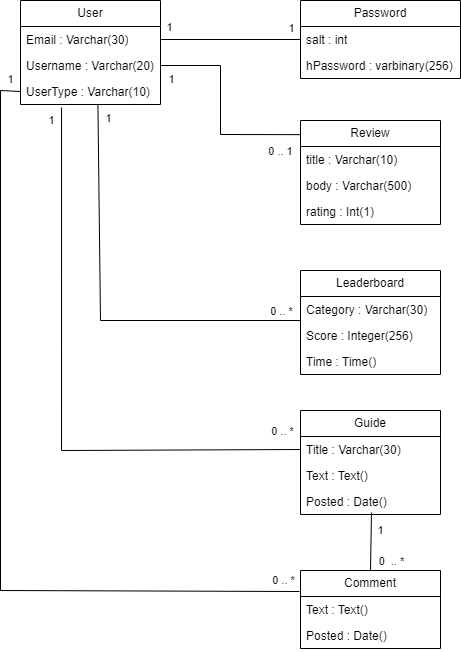
\includegraphics[scale=0.5]{figs/databaseUML.png}
    \caption{Database UML}
    \label{fig:1}
\end{figure*}

\begin{figure*}[!b]
    \centering
    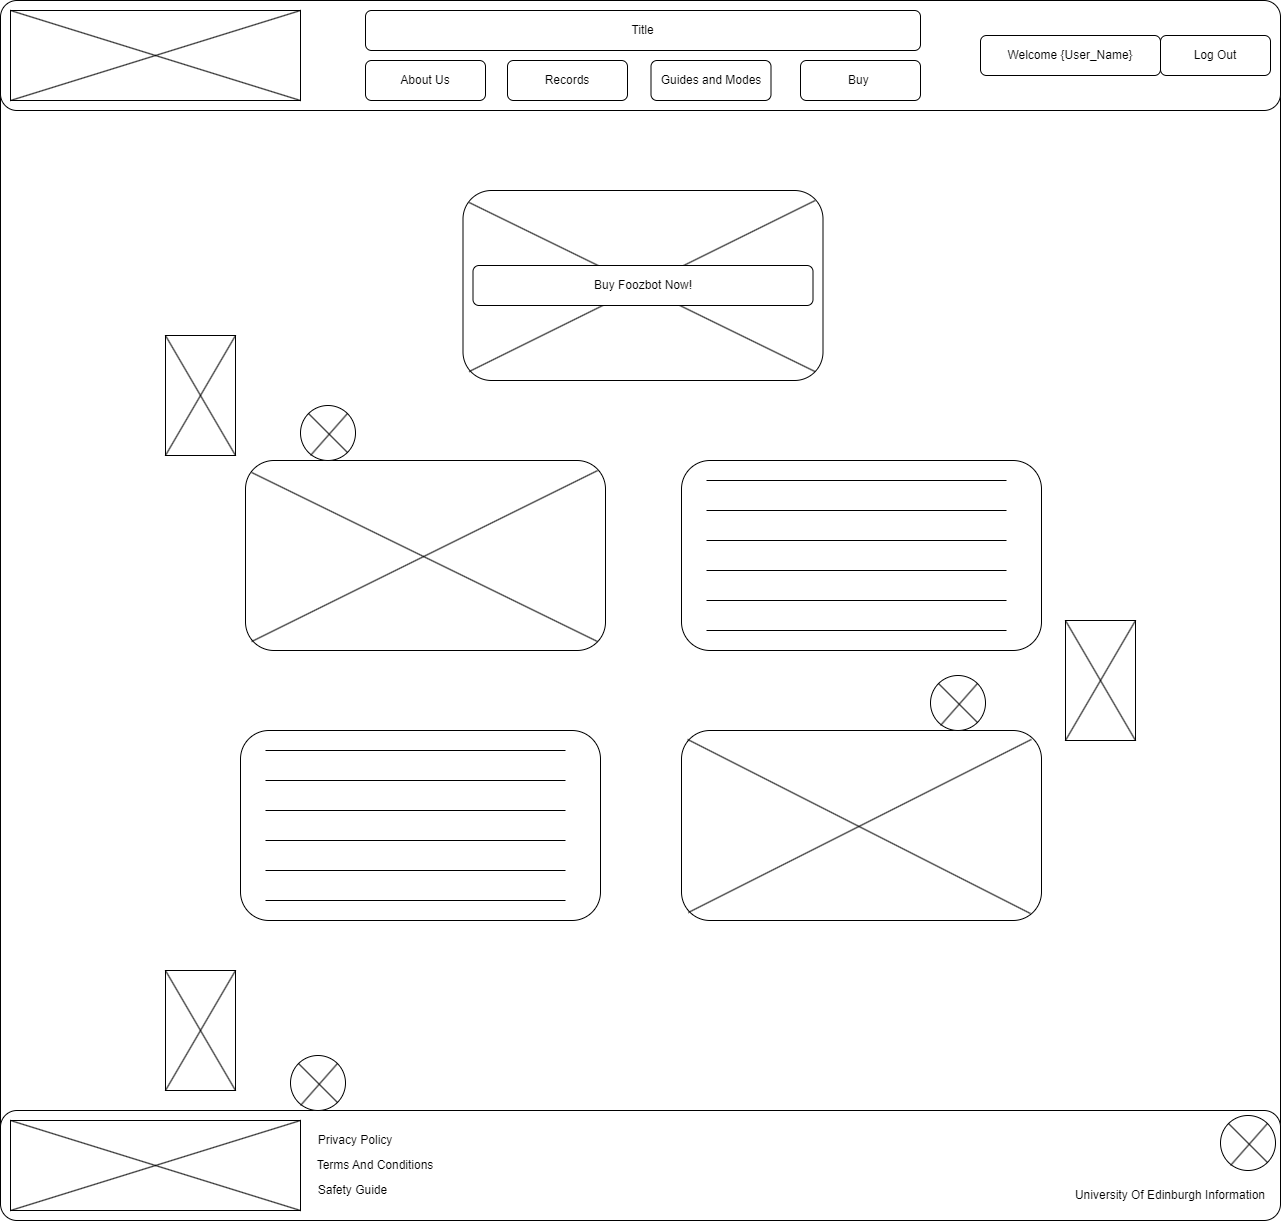
\includegraphics[width=10cm]{figs/homepage.png}
    \caption{Homepage design}
    \label{fig:2}
\end{figure*}

\bibliography{refs}

\end{document} 

